\documentclass[12pt, a4paper, oneside]{article}

\usepackage{fontspec}
\usepackage[polish]{babel}
\usepackage{geometry}
\usepackage{graphicx}
\usepackage{booktabs}
\usepackage{array}
\usepackage{longtable}
\usepackage{hyperref}
\usepackage{float}
\usepackage{enumitem}
\usepackage{xcolor}
\usepackage{minted}
\usepackage{caption}

\geometry{margin=2.5cm}

\definecolor{codebg}{RGB}{245,245,245}

\setminted{
  bgcolor=codebg,
  fontsize=\footnotesize,
  linenos=true,
  breaklines=true,
  frame=single,
  framesep=4pt,
  numbersep=6pt,
  tabsize=4,
  autogobble
}

\newcommand{\codecaption}[1]{\par\vspace{-0.4em}\noindent\small\textit{#1}\par\vspace{0.3em}}

\hypersetup{
    colorlinks=true,
    linkcolor=blue!60!black,
    urlcolor=blue!60!black,
    pdftitle={Sprawozdanie końcowe -- Aplikacja do zarządzania zadaniami},
    pdfauthor={Bartłomiej Karkoszka, Rafał Grot, Filip Stępień}
}

\title{\LARGE\bfseries Sprawozdanie końcowe\\[0.4cm]
  {\Large Aplikacja webowa do zarządzania zadaniami}}
\author{Bartłomiej Karkoszka \and Rafał Grot \and Filip Stępień}
\date{Przedmiot: Modelowanie i Analiza Systemów Informatycznych\\Grupa: 1ID21A}

\raggedbottom
\sloppy
\emergencystretch=3em

\begin{document}

\maketitle
\thispagestyle{empty}

\vspace{1.0cm}

\tableofcontents
\newpage

% ============================================================
% 1. OPIS TEMATU PROJEKTU
% ============================================================
\section{Opis tematu projektu}

Tematem projektu jest \textbf{webowa aplikacja do zarządzania zadaniami}
(typu \emph{TODO list}) przeznaczona dla użytkowników indywidualnych.
System pozwala zalogowanemu użytkownikowi tworzyć, edytować, oznaczać
statusem oraz usuwać własne zadania, a~także przeglądać podsumowanie
statystyczne w~formie panelu \emph{dashboard}. Każde zadanie posiada
tytuł, opcjonalny opis, status realizacji, poziom priorytetu oraz
opcjonalny termin wykonania.

Projekt został zrealizowany jako pełnoprawna aplikacja typu
\emph{full-stack}: część kliencka (SPA w~React 19) komunikuje się
poprzez REST API z~częścią serwerową napisaną w~języku Go. Funkcje
uwierzytelniania i~autoryzacji zostały delegowane do zewnętrznego
serwisu \textbf{Keycloak} (protokoły OAuth2 / OpenID Connect),
co eliminuje konieczność przechowywania haseł w~bazie aplikacji.
Cały system jest dostarczony jako zestaw kontenerów Docker, dzięki
czemu jego uruchomienie wymaga jedynie posiadania środowiska
\texttt{docker compose}.

% ============================================================
% 2. SKŁAD ZESPOŁU
% ============================================================
\section{Skład zespołu}

\begin{itemize}
  \item \textbf{Bartłomiej Karkoszka} -- modelowanie, dokumentacja, frontend,
  \item \textbf{Rafał Grot} -- backend (Go), baza danych, integracja z~Keycloak, frontend,
  \item \textbf{Filip Stępień} -- frontend (React, Redux Toolkit), warstwa prezentacji.
\end{itemize}

Wszyscy członkowie zespołu uczestniczyli również w~przygotowaniu
dokumentacji projektowej oraz w~przeglądach kodu (\emph{code review})
realizowanych poprzez \emph{pull requesty} w~repozytorium Git.

% ============================================================
% 3. ZAŁOŻENIA PROJEKTOWE
% ============================================================
\section{Założenia projektowe}

\subsection{Założenia funkcjonalne}
\begin{itemize}
  \item Rejestracja, logowanie i~wylogowanie użytkownika realizowane przez serwis Keycloak.
  \item Tworzenie zadania z~tytułem, opisem, priorytetem i~terminem realizacji.
  \item Edycja i~usuwanie własnych zadań użytkownika.
  \item Zmiana statusu zadania (Do zrobienia / W~trakcie / Zrobione).
  \item Filtrowanie listy zadań po statusie oraz priorytecie.
  \item Panel \emph{dashboard} z~podsumowaniem liczby zadań w~poszczególnych statusach.
\end{itemize}

\subsection{Założenia niefunkcjonalne}
\begin{itemize}
  \item Responsywny interfejs użytkownika (desktop, tablet, mobile).
  \item Bezpieczeństwo: hasła użytkowników \textbf{nie są} przechowywane
        w~bazie aplikacji -- uwierzytelnianie poprzez Keycloak,
        autoryzacja oparta o~tokeny JWT weryfikowane przez JWKS.
  \item Łatwe wdrożenie poprzez \texttt{docker compose} -- jedna komenda
        uruchamia bazę danych, Keycloak oraz Adminera.
  \item Wersjonowanie kodu w~Git (repozytorium monorepo).
  \item Statyczne typowanie zarówno po stronie backendu (Go) jak i~frontendu
        (TypeScript), generowane zapytania SQL (\texttt{sqlc}) oraz generowany
        klient REST (\texttt{Orval}) zapewniają spójność typów między warstwami.
\end{itemize}

\subsection{Założenia technologiczne}
\begin{itemize}
  \item \textbf{Frontend:} React 19, TypeScript, Vite, Tailwind CSS v4,
        shadcn/ui, React Router v7, Redux Toolkit (z~\texttt{createEntityAdapter}).
  \item \textbf{Backend:} Go (router \texttt{chi}, generator zapytań \texttt{sqlc},
        migracje \texttt{goose}, logger \texttt{slog}, dokumentacja \texttt{swaggo}).
  \item \textbf{Baza danych:} PostgreSQL 16.
  \item \textbf{Uwierzytelnianie:} Keycloak 26.2 (OAuth2 / OIDC, PKCE, JWKS).
  \item \textbf{Konteneryzacja:} Docker, Docker Compose.
\end{itemize}

W~stosunku do kamienia milowego~I jedyną istotną zmianą jest zastąpienie
zaplanowanego Spring Boot (Java) przez Go po stronie backendu -- decyzja
podyktowana chęcią wypróbowania języka w~praktyce.

% ============================================================
% 4. ARCHITEKTURA I DIAGRAMY
% ============================================================
\section{Architektura i diagramy}

\subsection{Diagram przypadków użycia}
Diagram przedstawia interakcje aktora \emph{Użytkownik} (umieszczonego
wewnątrz granicy systemu) z~aplikacją oraz powiązanie z~zewnętrznym
dostawcą tożsamości (Keycloak). Przypadek \emph{Synchronizuj profil
  użytkownika} (relacja \texttt{<<include>>}) odpowiada rzeczywistemu
mechanizmowi tworzenia rekordu w~tabeli \texttt{users} przy pierwszym
żądaniu autoryzowanym.

\begin{figure}[H]
  \centering
  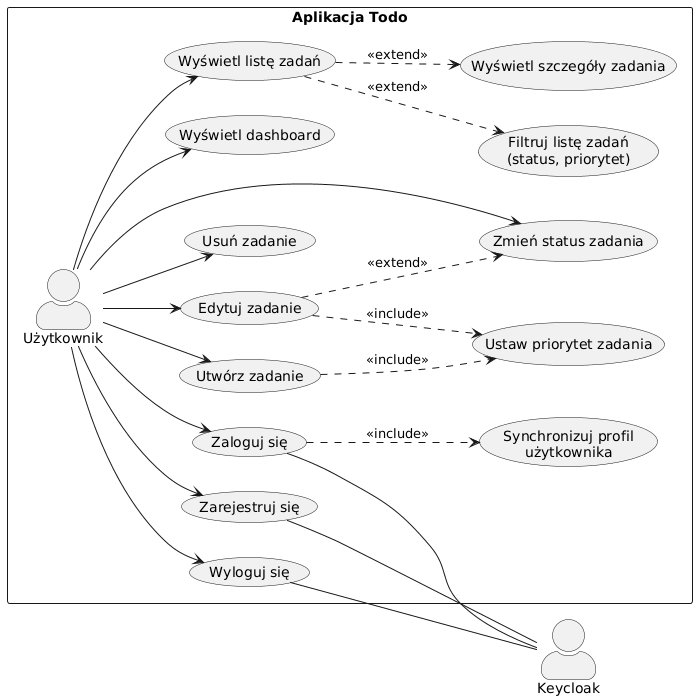
\includegraphics[width=0.85\textwidth]{diagrams/use_case_diagram.png}
  \caption{Diagram przypadków użycia}
\end{figure}

\subsection{Diagram klas (model dziedziny)}
Model dziedziny zawiera dwie główne encje: \texttt{User} oraz \texttt{Task},
powiązane relacją \emph{1 do 0..*}. Typy wyliczeniowe \texttt{TaskStatus}
(\texttt{todo}, \texttt{in\_progress}, \texttt{done}) oraz \texttt{TaskPriority}
(\texttt{low}, \texttt{medium}, \texttt{high}) zostały zaimplementowane jako
natywne typy enum w~PostgreSQL. Klasy pomocnicze \texttt{TaskFilters} oraz
\texttt{DashboardSummary} odpowiadają DTO obecnym w~kodzie.

\begin{figure}[H]
  \centering
  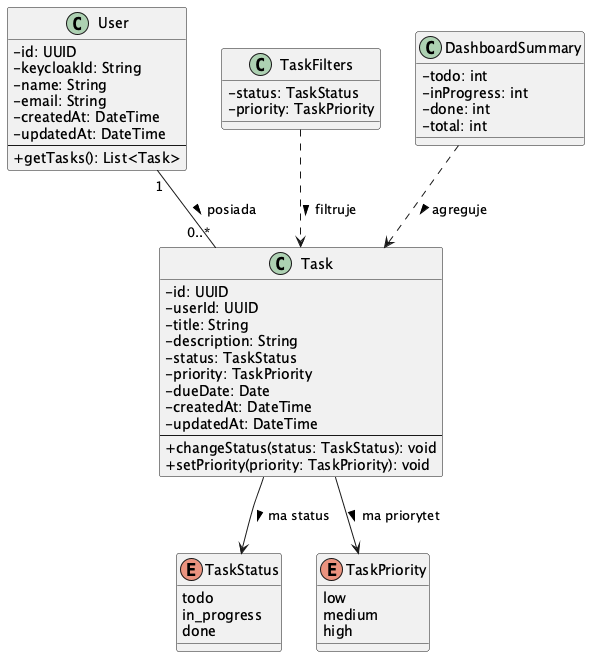
\includegraphics[width=0.80\textwidth]{diagrams/class_diagram.png}
  \caption{Diagram klas}
\end{figure}

\subsection{Diagram komponentów}
Diagram odzwierciedla rzeczywiste pakiety: po stronie frontendu wydzielony
jest \emph{Redux Store} (slice, thunki, selektory) oraz komponenty UI
(\texttt{Layout}, \texttt{TaskDialog}, \texttt{TaskItem}, \texttt{StatCard},
\texttt{ProfileMenu}). Po stronie backendu przedstawiono router \texttt{chi},
\texttt{AuthMiddleware} z~weryfikacją JWKS, handlery, warstwę serwisów
oraz wygenerowane przez \texttt{sqlc} \texttt{Queries}.

\begin{figure}[H]
  \centering
  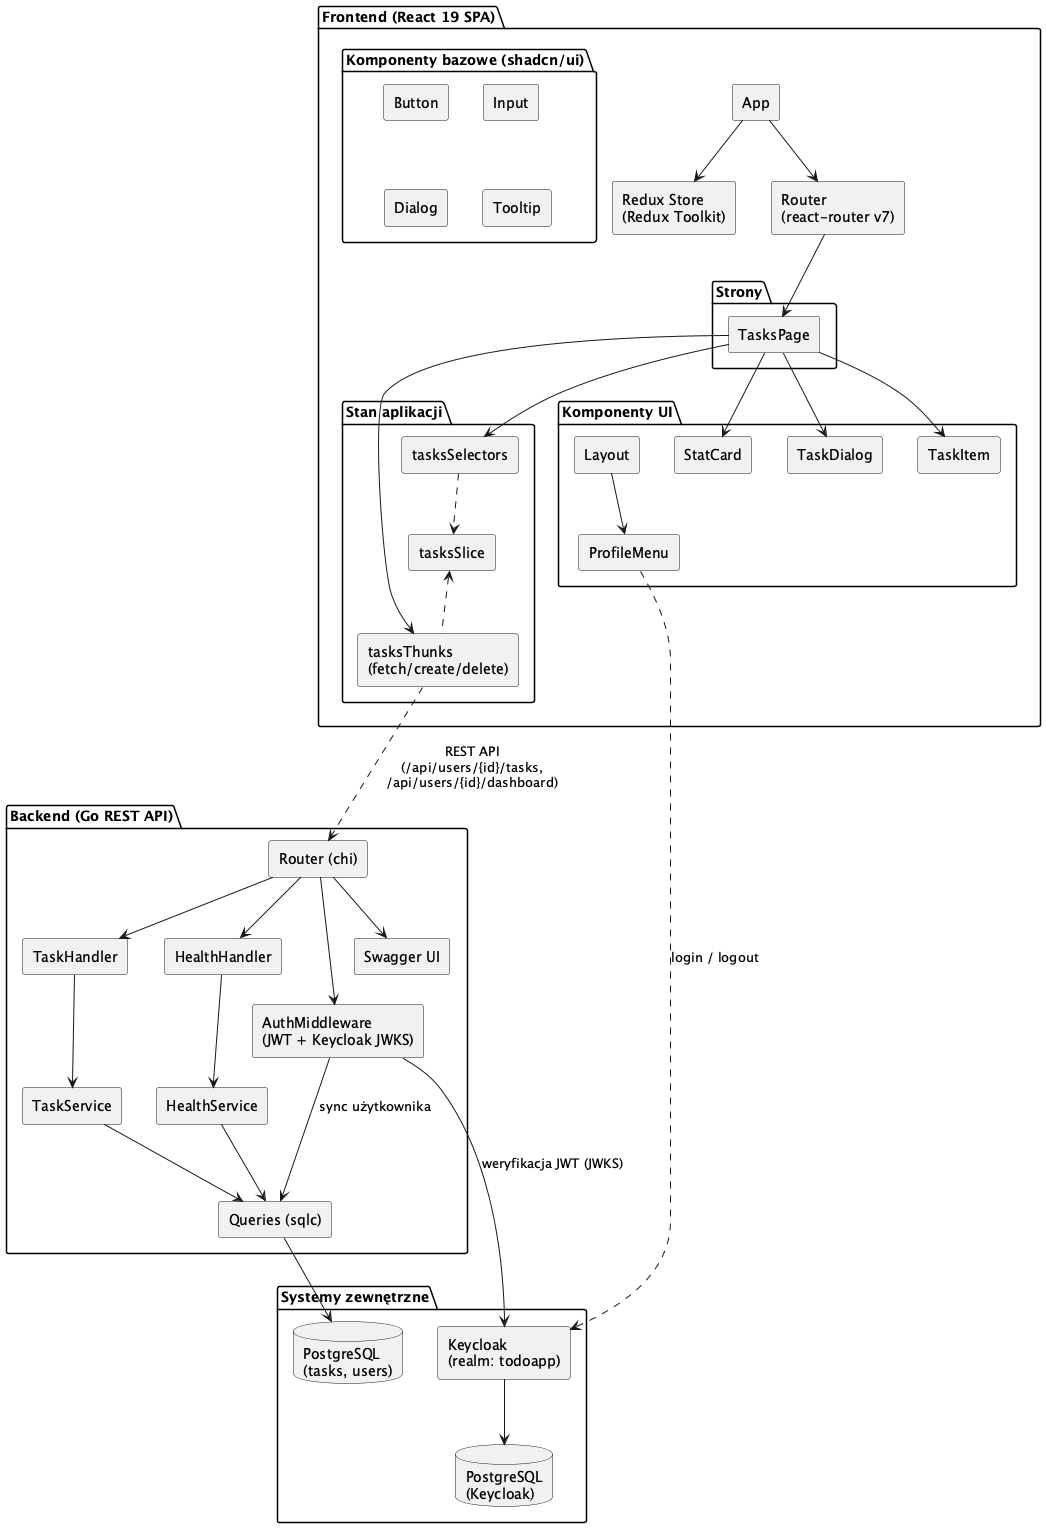
\includegraphics[width=\textwidth]{diagrams/component_diagram.png}
  \caption{Diagram komponentów}
\end{figure}

\subsection{Diagram warstw}
Architektura wpisuje się w~klasyczny model warstwowy: prezentacja
(React + Redux), API (chi, Swagger UI), logika (handlery, serwisy),
dostęp do danych (\texttt{sqlc}), dane (PostgreSQL) oraz przekrojowa
warstwa bezpieczeństwa (Keycloak, JWT).

\begin{figure}[H]
  \centering
  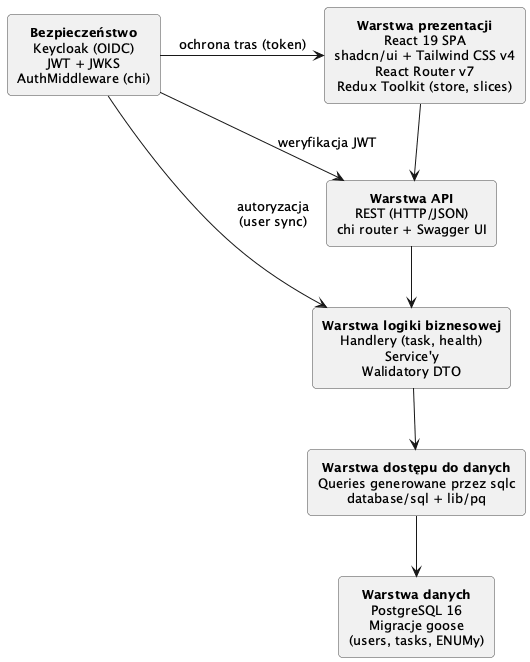
\includegraphics[width=0.72\textwidth]{diagrams/layer_diagram.png}
  \caption{Diagram warstw systemu}
\end{figure}

\subsection{Diagram sekwencji -- utworzenie zadania}
Diagram ilustruje pełny przepływ przez wszystkie warstwy systemu:
od interakcji w~UI, przez akcję Redux i~żądanie HTTP, weryfikację
tokenu, synchronizację użytkownika, walidację DTO, persystencję
w~bazie, aż po aktualizację stanu po stronie klienta.

\begin{figure}[H]
  \centering
  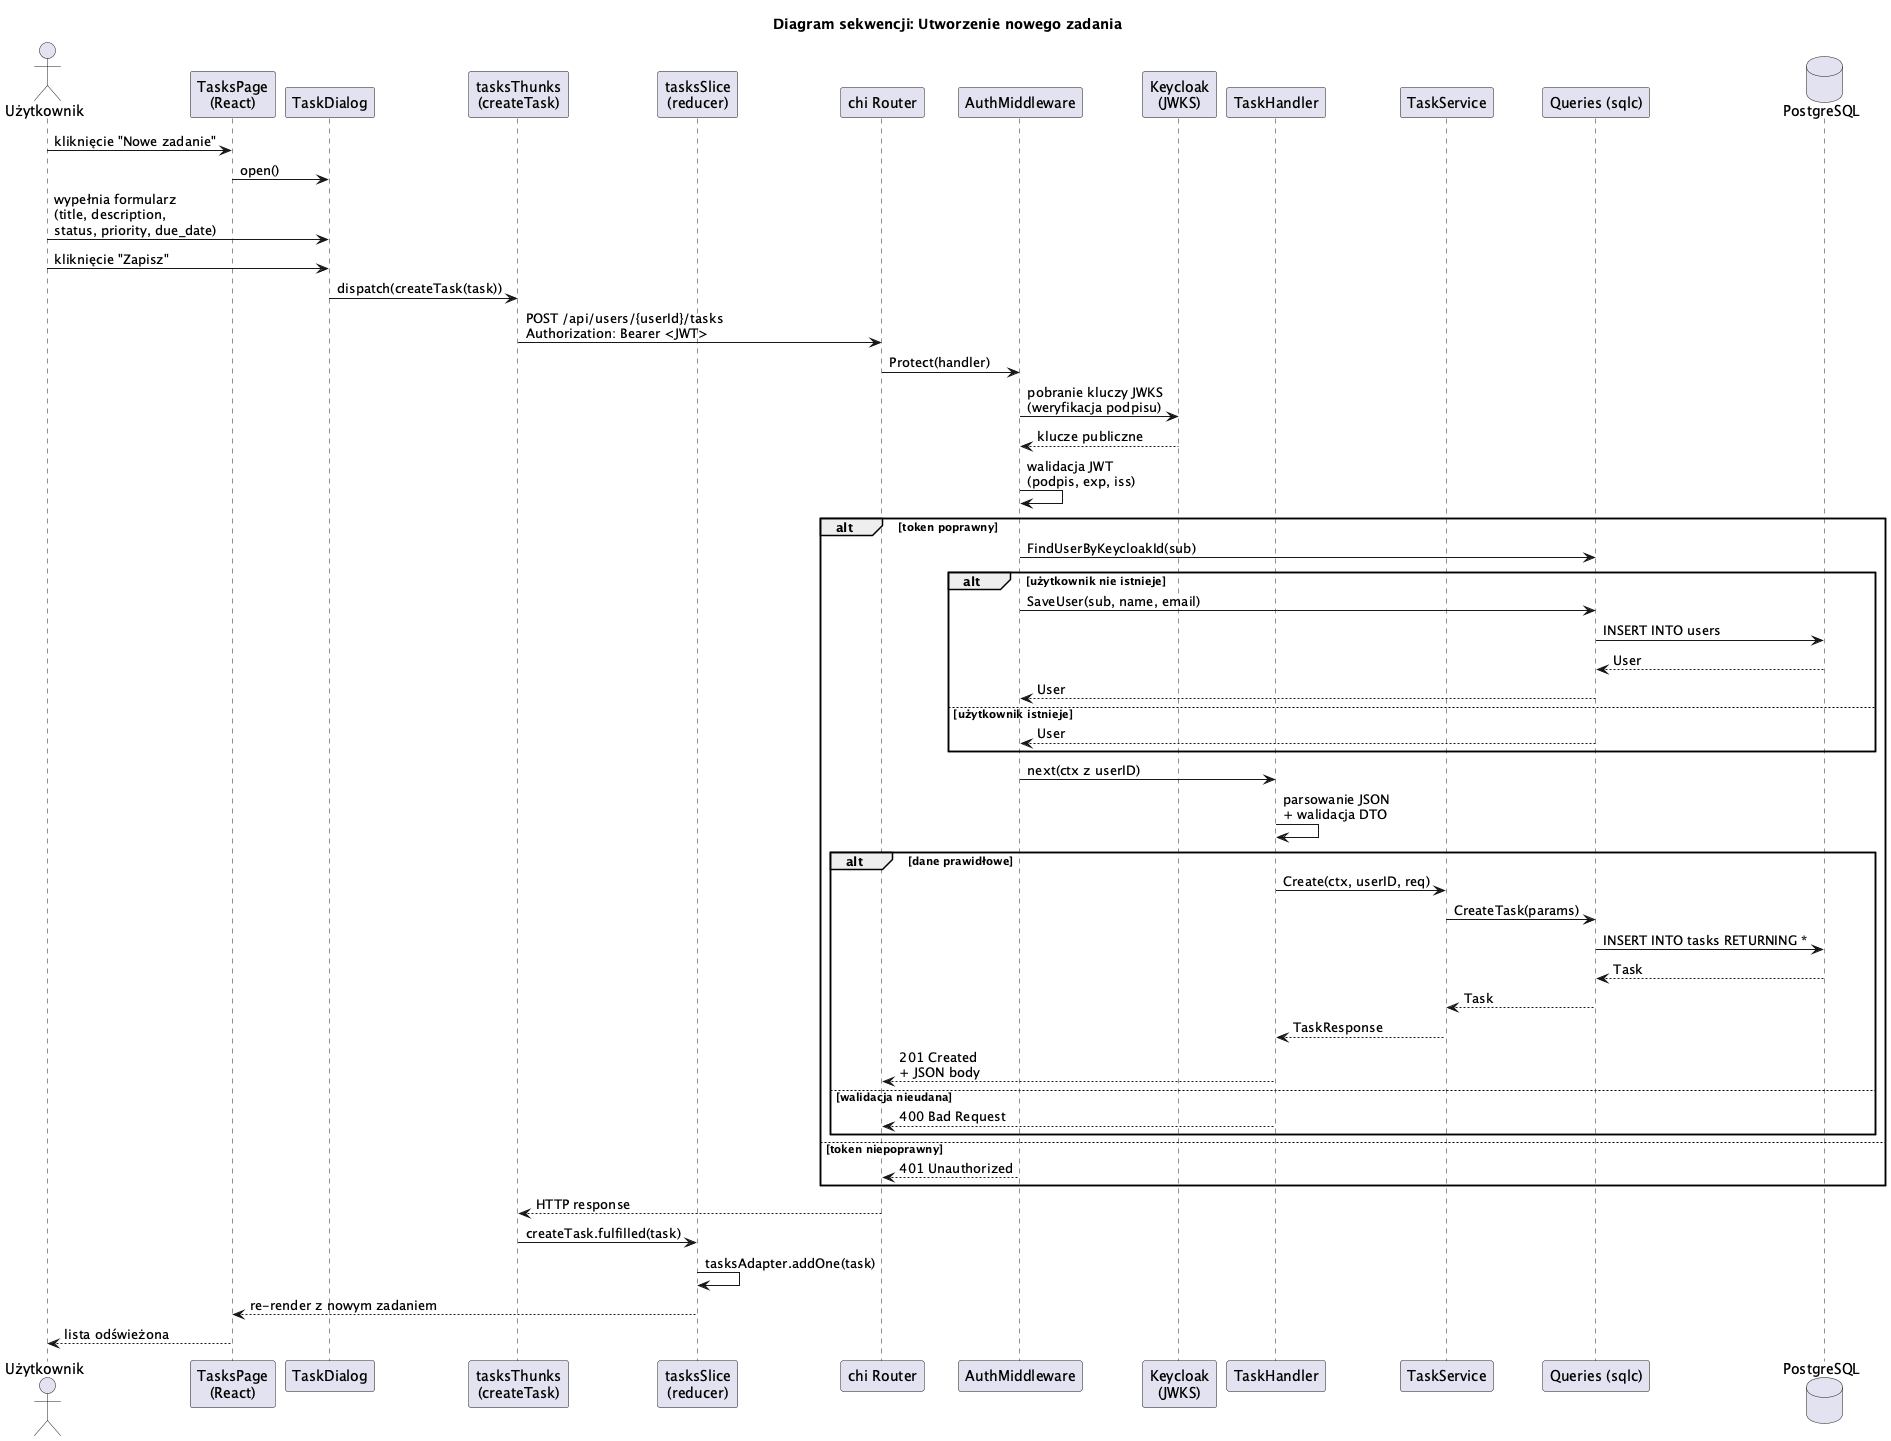
\includegraphics[width=\textwidth]{diagrams/sequence_diagram.png}
  \caption{Diagram sekwencji -- utworzenie nowego zadania}
\end{figure}

\subsection{Diagram aktywności}
Diagram aktywności pokazuje ogólną obsługę żądania zarządzania zadaniem
wraz z~punktami decyzyjnymi dla istotnych ścieżek błędu obecnych
w~implementacji: 401 (brak / niepoprawny token), 400 (błędne dane
wejściowe) oraz 404 (\texttt{sql.ErrNoRows}).

\begin{figure}[H]
  \centering
  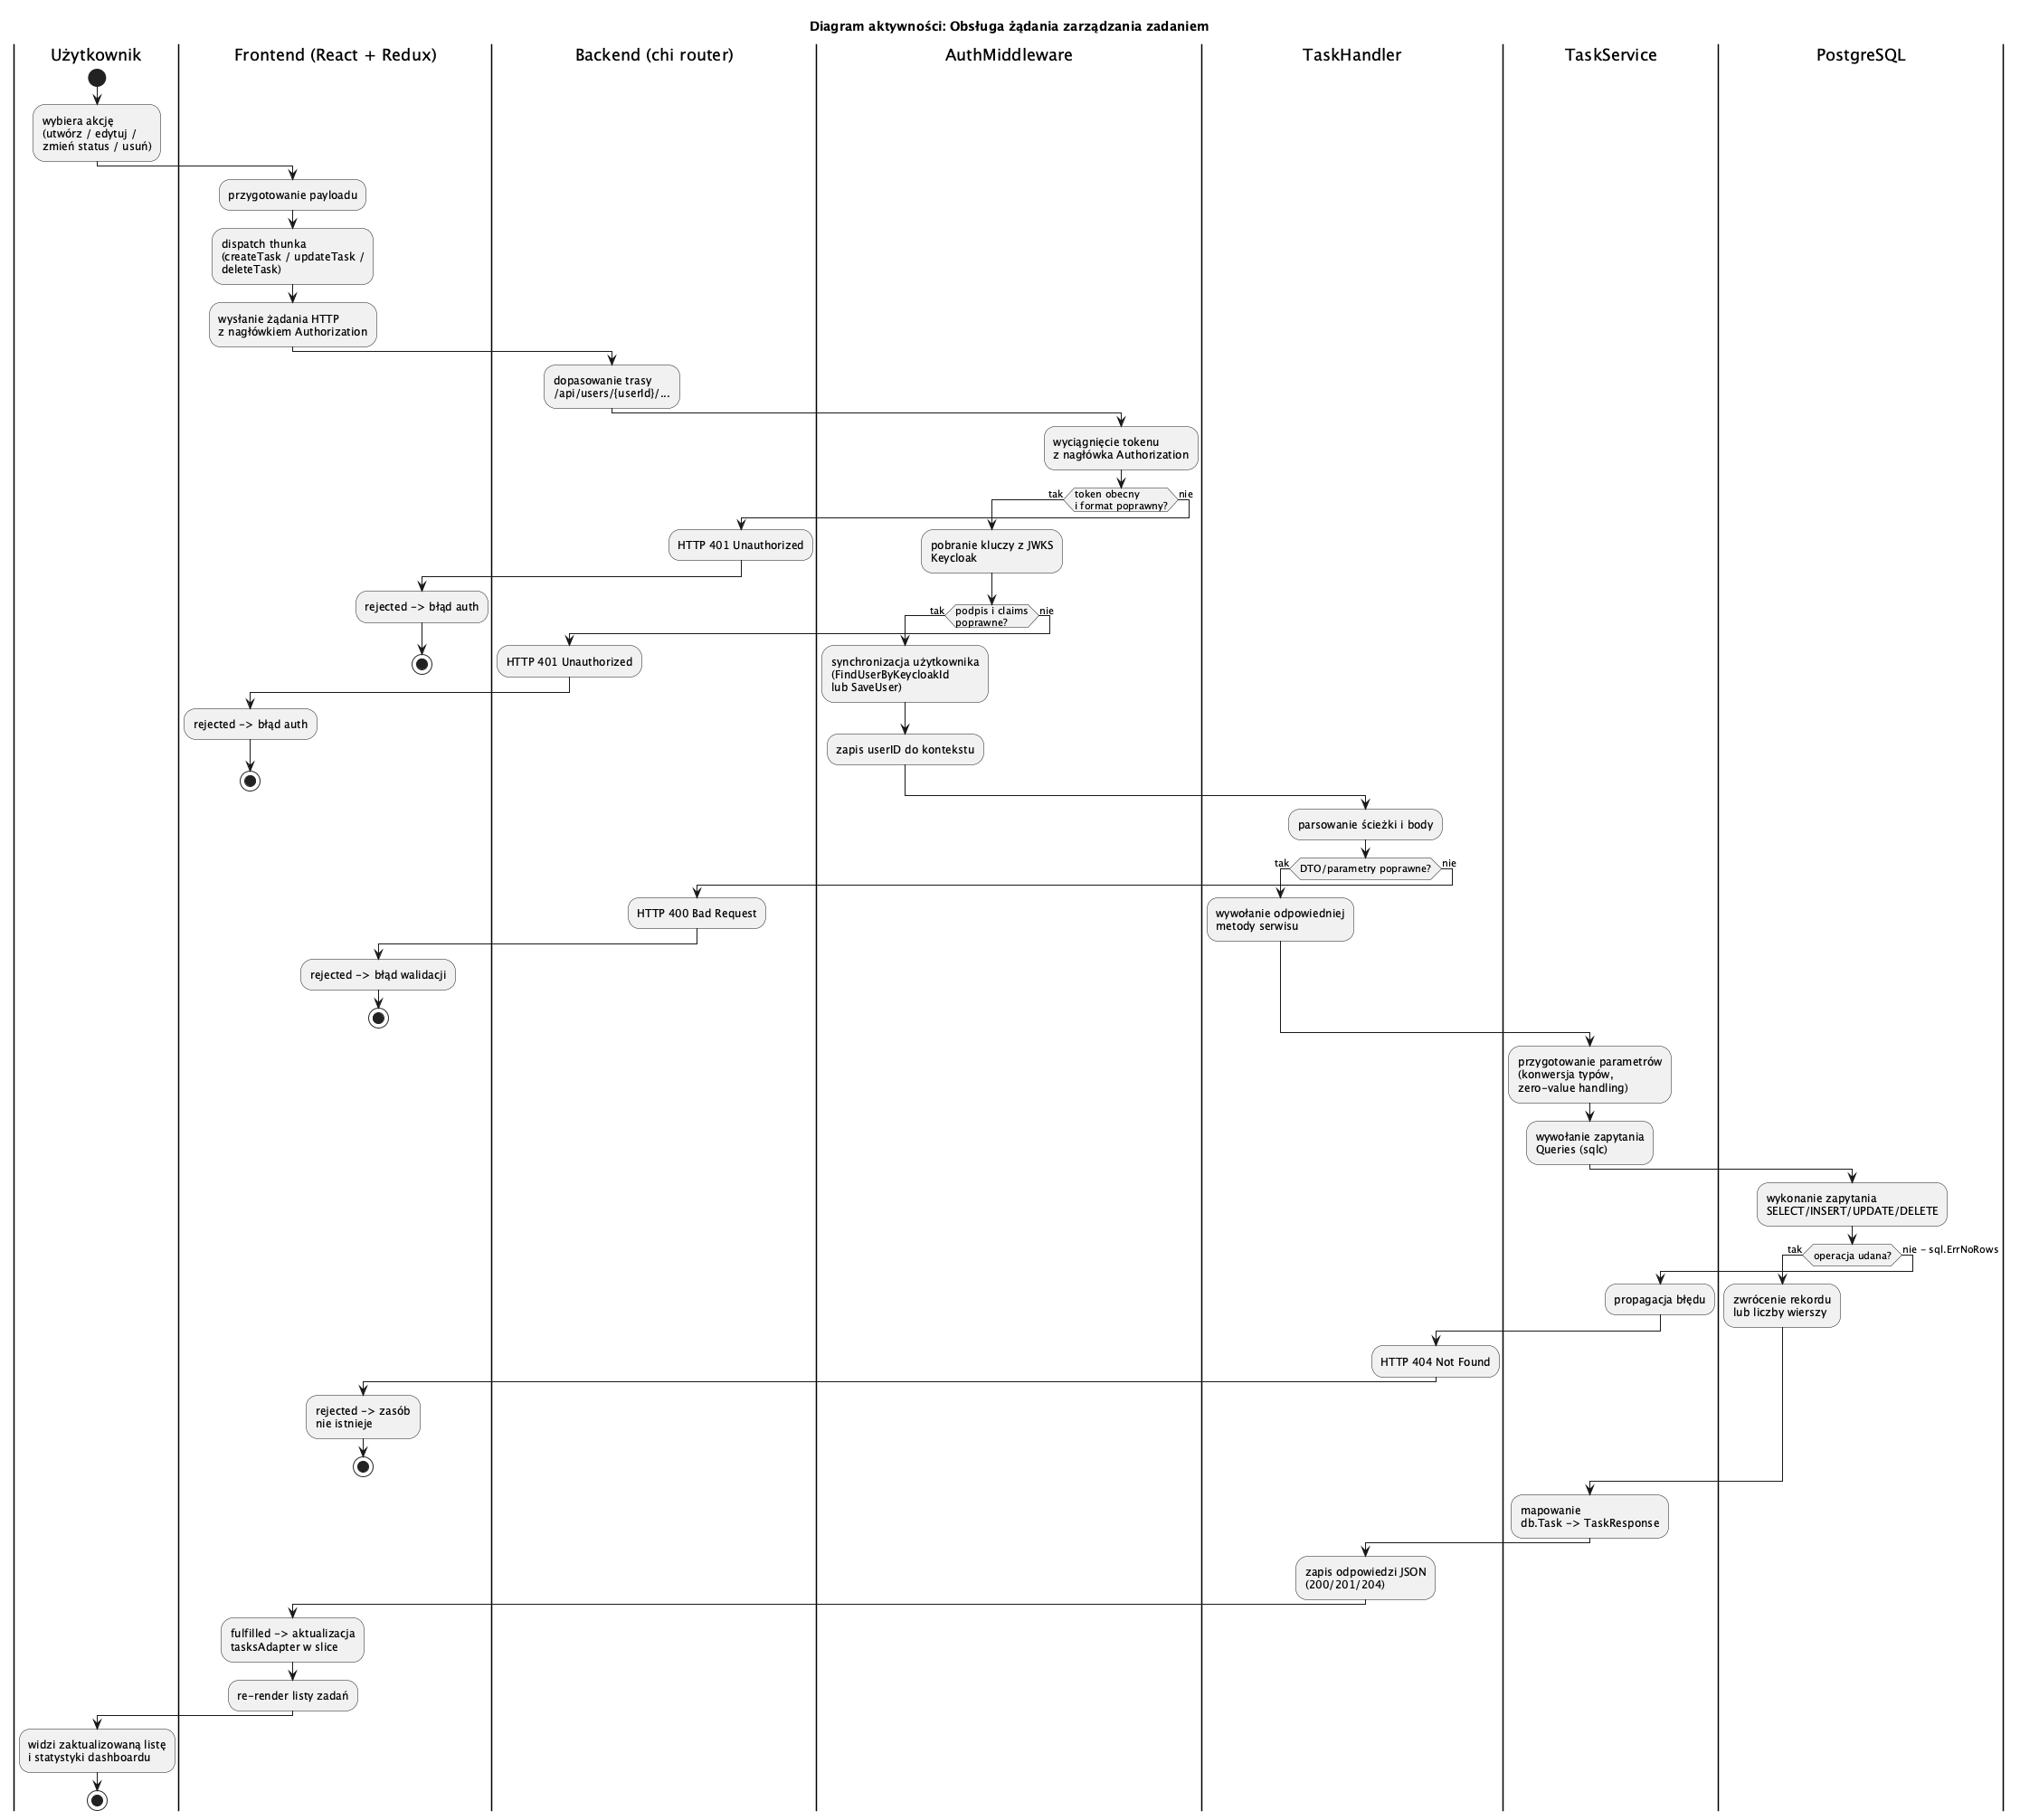
\includegraphics[width=\textwidth]{diagrams/activity_diagram.png}
  \caption{Diagram aktywności -- obsługa żądania zarządzania zadaniem}
\end{figure}

% ============================================================
% 5. GRAF ZALEŻNOŚCI MODUŁÓW
% ============================================================
\section{Graf zależności pomiędzy modułami}

System zorganizowany jest jako \emph{monorepo} z~dwoma aplikacjami:
\texttt{apps/task-api} (backend Go) oraz \texttt{apps/task-frontend}
(frontend React). Przedstawione poniżej grafy zostały wygenerowane
automatycznie z~kodu źródłowego: dla backendu narzędziem
\texttt{godepgraph} (analiza importów pakietów Go) renderowanym przez
Graphviz, dla frontendu narzędziem \texttt{madge} (analiza importów
plików TypeScript / TSX).

\subsection{Zależności w backendzie (Go)}

Graf zależności pomiędzy pakietami w~obrębie modułu
\texttt{task-api} (bez bibliotek zewnętrznych oraz standardowej
biblioteki Go).

\begin{figure}[H]
  \centering
  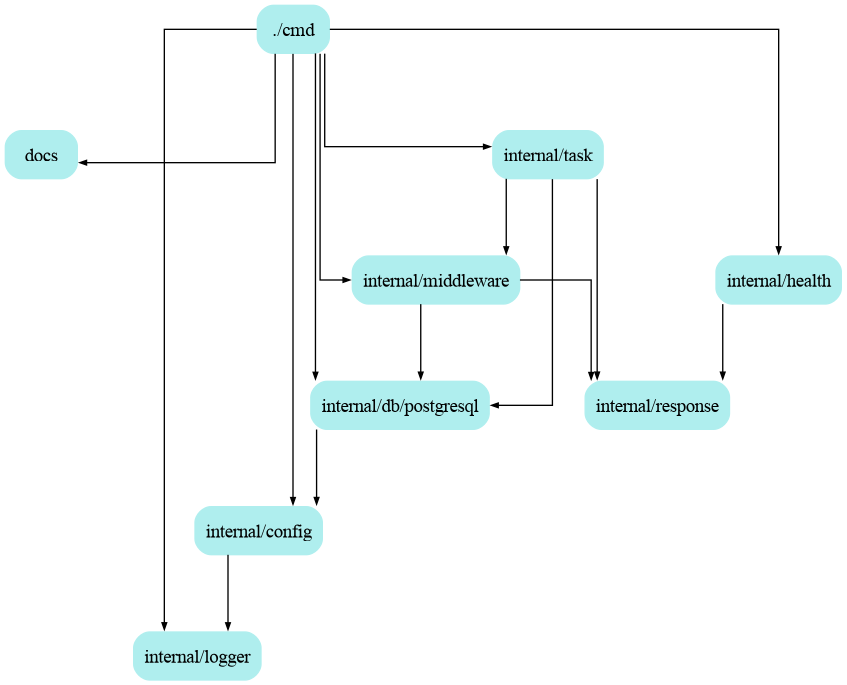
\includegraphics[width=\textwidth]{diagrams/backend_deps.png}
  \caption{Graf zależności pakietów backendu (\texttt{godepgraph} + Graphviz)}
\end{figure}

Punkt wejścia (\texttt{cmd}) zależy bezpośrednio od wszystkich
pakietów aplikacyjnych. Pakiet \texttt{internal/response} jest wspólną
zależnością warstwy HTTP (\texttt{middleware}, \texttt{task},
\texttt{health}). Warstwa danych (\texttt{internal/db/postgresql})
jest wykorzystywana zarówno przez \texttt{middleware} (synchronizacja
profilu użytkownika), jak i~przez \texttt{task} (CRUD zadań).

\subsection{Zależności we frontendzie (React + Redux)}

Graf zależności modułów frontendu zaczyna się od \texttt{main.tsx}
i~rozgałęzia się na trzy poddrzewa: routing (\texttt{router.tsx} --
\texttt{pages/}), warstwę uwierzytelniania (\texttt{providers/auth-provider.tsx})
oraz store Redux (\texttt{lib/store.ts} -- \texttt{state/tasks/}).
W~grafie pominięto komponenty bazowe biblioteki shadcn/ui
(\texttt{components/ui/}) oraz pomocniczy plik \texttt{lib/utils.ts}
celem zachowania czytelności rysunku.

\begin{figure}[H]
  \centering
  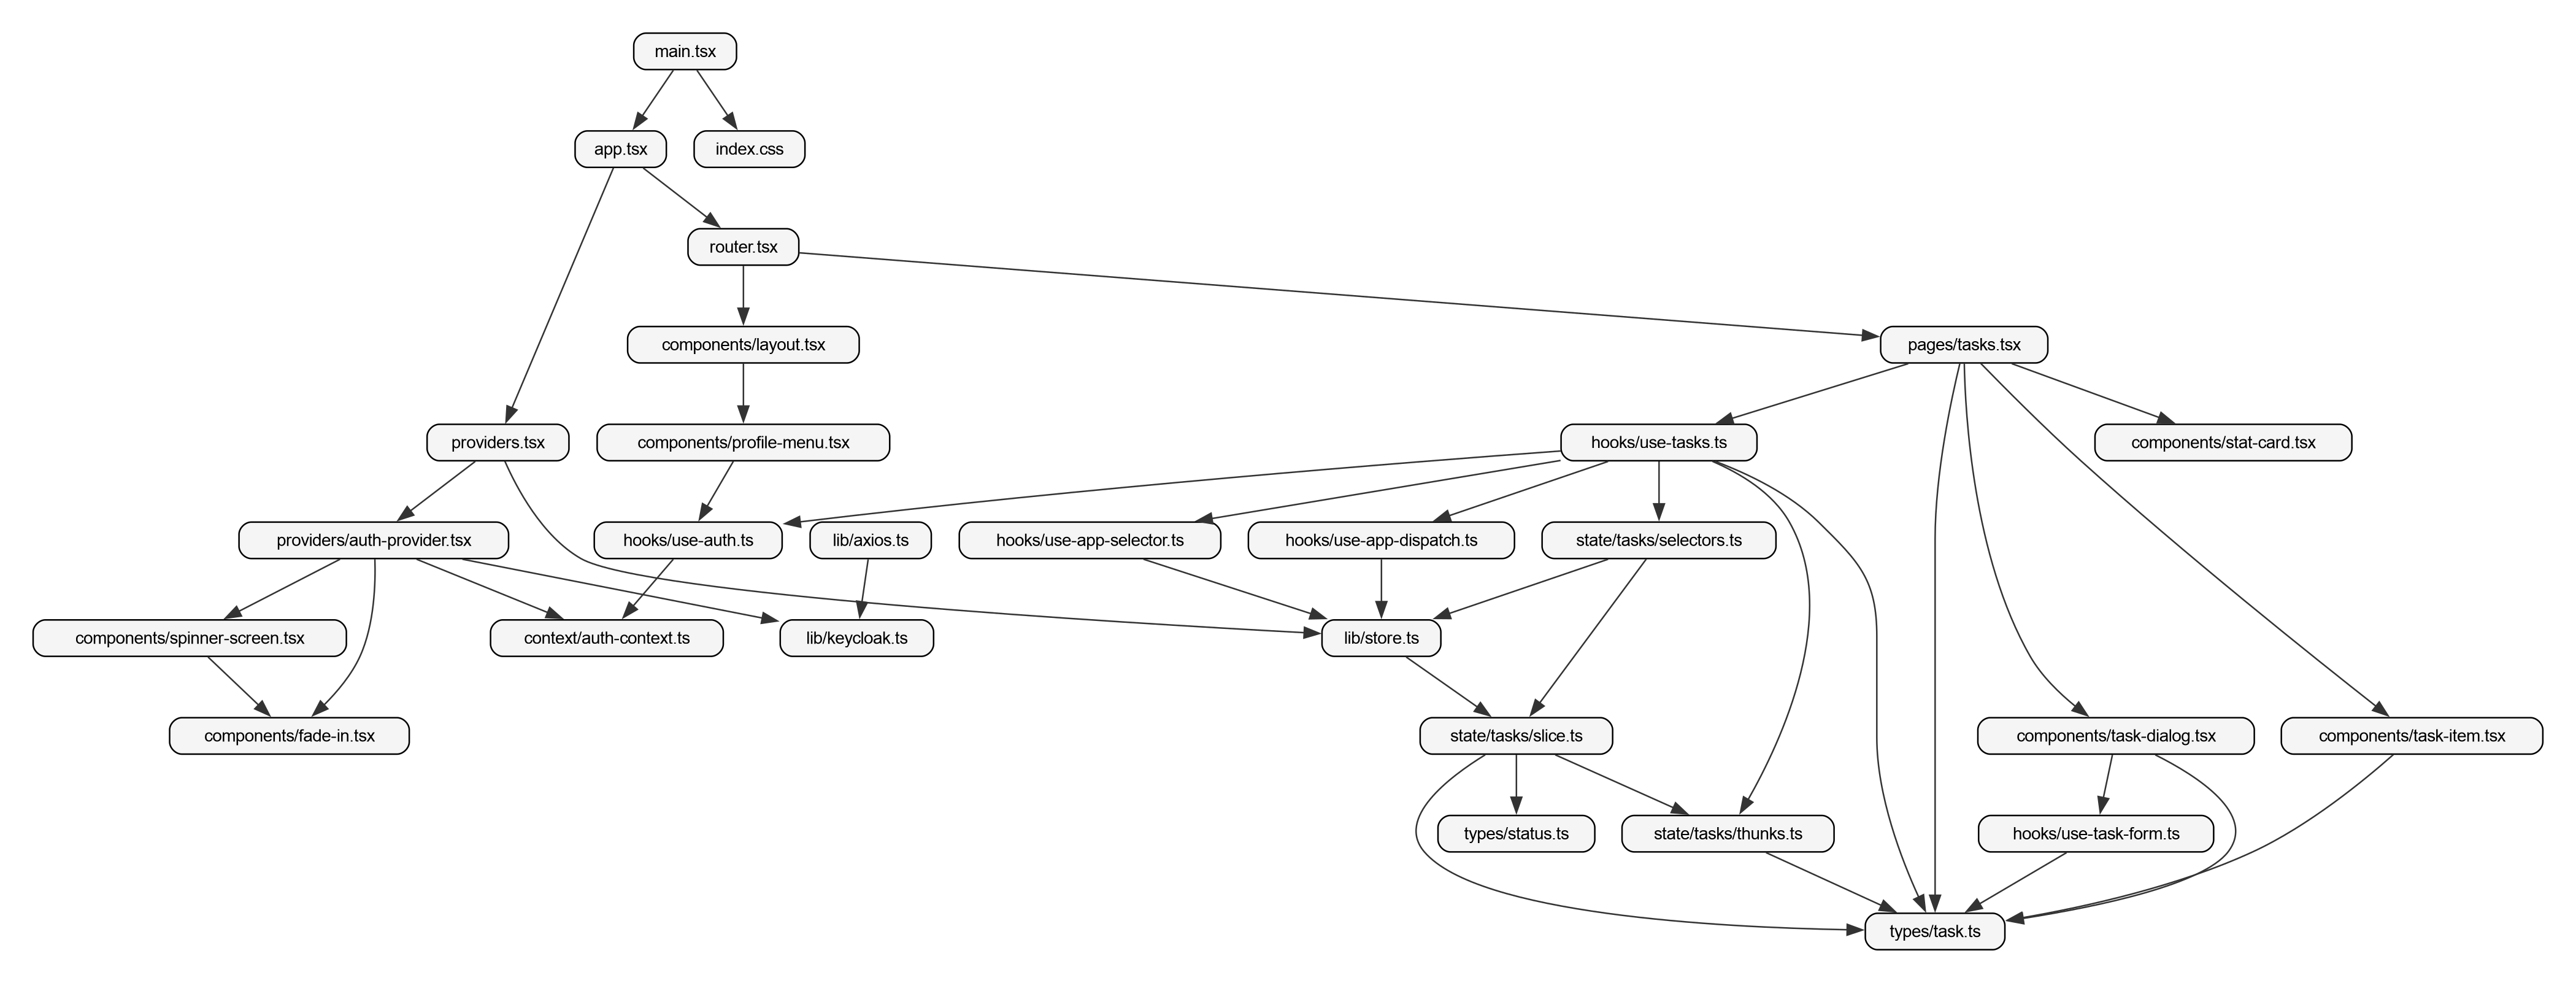
\includegraphics[width=\textwidth]{diagrams/frontend_deps.png}
  \caption{Graf zależności modułów frontendu (\texttt{madge} + Graphviz)}
\end{figure}

\subsection{Komunikacja między aplikacjami}
\begin{itemize}
  \item \textbf{Frontend -- Backend}: komunikacja po REST/JSON pod
        endpointami \texttt{/api/users/\{id\}/tasks} oraz
        \texttt{/api/users/\{id\}/dashboard}. Klient HTTP (\texttt{axios})
        automatycznie dołącza nagłówek \texttt{Authorization: Bearer <JWT>}.
  \item \textbf{Frontend -- Keycloak}: przepływ OAuth2 / OIDC w~wariancie
        \emph{authorization code} z~PKCE, realizowany przez bibliotekę
        \texttt{keycloak-js}.
  \item \textbf{Backend -- Keycloak}: backend pobiera klucze publiczne
        z~JWKS pod ścieżką \texttt{/realms/todoapp/protocol/openid-connect/certs}
        i~weryfikuje podpis tokenów JWT przy pomocy biblioteki
        \texttt{MicahParks/keyfunc}.
  \item \textbf{Backend -- PostgreSQL}: pula połączeń \texttt{database/sql},
        zapytania generowane przez \texttt{sqlc}.
\end{itemize}

% ============================================================
% 6. METRYKI KODU
% ============================================================
\section{Metryki kodu}\label{sec:metryki}

Metryki zostały zebrane przy pomocy narzędzi \texttt{tokei} (liczba
plików i~linii kodu) oraz \texttt{gocyclo} (cyklomatyczna złożoność
funkcji w~języku Go).

% Auto-generated by doc/scripts/gen-metrics.sh
\newcommand{\metricsAvgCC}{2,55}


\subsection{Liczba plików i~linii kodu (tokei)}

\inputminted[fontsize=\footnotesize,linenos=false,frame=single,breaklines=true]{text}{generated/tokei.txt}

\subsection{Cyklomatyczna złożoność (gocyclo)}

Średnia cyklomatyczna złożoność funkcji w~kodzie Go wynosi
\textbf{\metricsAvgCC}. Zdecydowana większość funkcji ma złożoność
1--3 (wartości uznawane za \emph{trywialne} w~skali McCabe'a).
Poniżej surowy wynik \texttt{gocyclo -top 15} (kolumny: złożoność,
pakiet, funkcja, plik z~numerem linii):

\inputminted[fontsize=\footnotesize,linenos=false,frame=single,breaklines=true]{text}{generated/gocyclo.txt}

\subsection{Frontend -- struktura}
Po stronie React zaimplementowano:
\begin{itemize}
  \item \textbf{1 stronę} (\texttt{TasksPage}),
  \item \textbf{7 komponentów aplikacyjnych} (\texttt{Layout}, \texttt{TaskDialog},
        \texttt{TaskItem}, \texttt{ProfileMenu}, \texttt{StatCard},
        \texttt{FadeIn}, \texttt{SpinnerScreen}),
  \item \textbf{13 komponentów UI} z~biblioteki shadcn/ui,
  \item \textbf{6 customowych hooków} (\texttt{useTasks}, \texttt{useTaskForm},
        \texttt{useAuth}, \texttt{useAppDispatch}, \texttt{useAppSelector},
        \texttt{useMobile}),
  \item \textbf{1 slice Redux} z~\texttt{createEntityAdapter} oraz
        \textbf{4 asynchroniczne thunki} (\texttt{fetchTasks},
        \texttt{createTask}, \texttt{updateTask}, \texttt{deleteTask}).
\end{itemize}

% ============================================================
% 7. STAN IMPLEMENTACJI I LISTA ENDPOINTÓW
% ============================================================
\section{Stan implementacji}

\subsection{Struktura repozytorium}
\begin{minted}[linenos=false,fontsize=\scriptsize]{text}
todoapp/
|-- apps/
|   |-- task-api/             # backend Go (REST API)
|   |   |-- cmd/              # main.go, api.go - bootstrap aplikacji
|   |   `-- internal/
|   |       |-- config/       # parametry srodowiskowe
|   |       |-- db/postgresql # modele, queries (sqlc), migracje
|   |       |-- health/       # endpoint /health
|   |       |-- logger/       # slog wrapper
|   |       |-- middleware/   # AuthMiddleware (JWT, JWKS)
|   |       |-- response/     # pomocnicze pisanie JSON
|   |       `-- task/         # handler, service, dto
|   `-- task-frontend/        # frontend React (SPA)
|       `-- src/
|           |-- components/   # Layout, TaskDialog, TaskItem, ...
|           |-- pages/        # TasksPage
|           |-- hooks/        # custom hooks
|           |-- state/tasks/  # slice, thunks, selectors
|           |-- providers/    # AuthProvider
|           |-- lib/          # store, axios, keycloak, env
|           `-- generated/    # Orval - klient REST
|-- docker/keycloak/realm.json
|-- docker-compose.yml
|-- flake.nix
`-- Taskfile.yml
\end{minted}
\codecaption{Struktura repozytorium}

\subsection{Lista endpointów REST}
Wszystkie endpointy są zabezpieczone middleware \texttt{Protect}
wymagającym nagłówka \texttt{Authorization: Bearer <JWT>} i~udostępnione
pod prefiksem \texttt{/api} (konfigurowalnym przez zmienną
\texttt{API\_BASE\_PATH}).

\begingroup
\setlength{\tabcolsep}{4pt}
\renewcommand{\arraystretch}{1.15}
\begin{longtable}{@{}>{\raggedright\arraybackslash}p{1.6cm} >{\raggedright\arraybackslash\ttfamily\small}p{5.3cm} >{\raggedright\arraybackslash}p{4.6cm} >{\raggedright\arraybackslash}p{2.6cm}@{}}
  \toprule
  \textbf{Metoda} & \textbf{\normalfont\rmfamily Ścieżka} & \textbf{Opis}                      & \textbf{Kody}           \\
  \midrule
  \endhead
  GET             & /health                               & Stan aplikacji i~bazy danych       & 200, 401, 500           \\
  GET             & /users/\{userId\}/tasks               & Lista zadań użytkownika z~filtrami & 200, 400, 401, 500      \\
  POST            & /users/\{userId\}/tasks               & Utworzenie nowego zadania          & 201, 400, 401, 500      \\
  GET             & /users/\{userId\}/tasks/\{id\}        & Szczegóły pojedynczego zadania     & 200, 400, 401, 404, 500 \\
  PUT             & /users/\{userId\}/tasks/\{id\}        & Aktualizacja zadania               & 200, 400, 401, 404, 500 \\
  DELETE          & /users/\{userId\}/tasks/\{id\}        & Usunięcie zadania                  & 204, 400, 401, 404, 500 \\
  GET             & /users/\{userId\}/dashboard           & Statystyki zadań użytkownika       & 200, 400, 401, 500      \\
  \bottomrule
\end{longtable}
\endgroup

\subsection{Schemat bazy danych}
Migracje (\texttt{goose}) tworzą tabele \texttt{users} i~\texttt{tasks}
oraz typy wyliczeniowe \texttt{task\_status} (\texttt{todo},
\texttt{in\_progress}, \texttt{done}) i~\texttt{task\_priority}
(\texttt{low}, \texttt{medium}, \texttt{high}). Tabela \texttt{tasks}
posiada klucz obcy \texttt{user\_id} z~kaskadowym usuwaniem oraz
znaczniki czasowe \texttt{created\_at} i~\texttt{updated\_at}.

% ============================================================
% 8. KLUCZOWE FRAGMENTY KODU
% ============================================================
\section{Kluczowe fragmenty kodu}

W~tej sekcji prezentujemy najistotniejsze fragmenty implementacji.

\subsection{Middleware uwierzytelniania (Go)}
Środkowy element warstwy bezpieczeństwa: pobiera klucze publiczne
z~Keycloaka (JWKS), weryfikuje podpis JWT, a~następnie synchronizuje
profil użytkownika z~lokalną bazą (rekord tworzony jest \emph{lazy}
przy pierwszym żądaniu autoryzowanym).

\begin{minted}{go}
func (m *AuthMiddleware) Protect(next http.Handler) http.Handler {
    return http.HandlerFunc(func(w http.ResponseWriter, r *http.Request) {
        tokenStr, ok := extractAuthToken(r)
        if !ok {
            response.Error(w, http.StatusUnauthorized, "Unauthorized")
            return
        }

        claims, ok := m.parseTokenClaims(tokenStr)
        if !ok {
            response.Error(w, http.StatusUnauthorized, "Unauthorized")
            return
        }

        uc := extractClaims(claims)

        user, err := m.syncUser(r.Context(), uc)
        if err != nil {
            response.Error(w, http.StatusInternalServerError, "Failed to sync user")
            return
        }

        ctx := context.WithValue(r.Context(), UserIDKey, user.ID)
        next.ServeHTTP(w, r.WithContext(ctx))
    })
}
\end{minted}
\codecaption{\texttt{internal/middleware/auth.go} -- weryfikacja JWT i synchronizacja użytkownika}

Funkcja \texttt{syncUser} implementuje wzorzec \emph{lazy provisioning}:
jeżeli użytkownik o~podanym \texttt{sub} (z~tokenu JWT) nie istnieje
jeszcze w~tabeli \texttt{users}, zostaje utworzony nowy rekord;
w~przeciwnym przypadku zwracany jest istniejący.

\begin{minted}{go}
func (m *AuthMiddleware) syncUser(ctx context.Context, uc userClaims) (db.User, error) {
    user, err := m.queries.FindUserByKeycloakId(ctx, uc.sub)
    if err != nil && !errors.Is(err, sql.ErrNoRows) {
        return db.User{}, err
    }

    if errors.Is(err, sql.ErrNoRows) {
        user, err = m.queries.SaveUser(ctx, db.SaveUserParams{
            KeycloakID: uc.sub,
            Name:       uc.name,
            Email:      uc.email,
        })
        if err != nil {
            return db.User{}, err
        }
    }

    return user, nil
}
\end{minted}
\codecaption{\texttt{internal/middleware/auth.go} -- \texttt{syncUser}}

\subsection{Warstwa serwisów -- tworzenie zadania (Go)}
Serwis odpowiada za parsowanie daty, mapowanie pól opcjonalnych
na typy \texttt{sql.NullString} / \texttt{sql.NullTime} oraz wywołanie
wygenerowanego przez \texttt{sqlc} zapytania.

\begin{minted}{go}
func (s *service) Create(ctx context.Context, userID uuid.UUID, req CreateTaskRequest) (TaskResponse, error) {
    params := db.CreateTaskParams{
        UserID:   userID,
        Title:    req.Title,
        Status:   db.TaskStatus(req.Status),
        Priority: db.TaskPriority(req.Priority),
    }

    if req.Description != nil {
        params.Description = sql.NullString{String: *req.Description, Valid: true}
    }

    if req.DueDate != nil {
        t, err := time.Parse(time.DateOnly, *req.DueDate)
        if err != nil {
            return TaskResponse{}, err
        }
        params.DueDate = sql.NullTime{Time: t, Valid: true}
    }

    task, err := s.queries.CreateTask(ctx, params)
    if err != nil {
        return TaskResponse{}, err
    }
    return toTaskResponse(task), nil
}
\end{minted}
\codecaption{\texttt{internal/task/service.go} -- \texttt{Create}}

\subsection{Walidacja DTO (Go)}
Walidacja wykonywana jest na poziomie handlera, przed wejściem do
warstwy serwisów. Każde DTO eksponuje metodę \texttt{Validate()},
która kompozycyjnie wykorzystuje wspólne funkcje pomocnicze
(\texttt{validateStatus}, \texttt{validatePriority}, \texttt{validateDueDate}).

\begin{minted}{go}
var (
    validStatuses   = map[string]struct{}{"todo": {}, "in_progress": {}, "done": {}}
    validPriorities = map[string]struct{}{"low": {}, "medium": {}, "high": {}}
)

func validateStatus(s string) error {
    if _, ok := validStatuses[s]; !ok {
        return errors.New("status must be one of: todo, in_progress, done")
    }
    return nil
}

func validateDueDate(d *string) error {
    if d == nil || *d == "" {
        return nil
    }
    if _, err := time.Parse(time.DateOnly, *d); err != nil {
        return errors.New("due_date must be in YYYY-MM-DD format")
    }
    return nil
}

func (r CreateTaskRequest) Validate() error {
    if r.Title == "" {
        return errors.New("title is required")
    }
    if err := validateStatus(r.Status); err != nil {
        return err
    }
    if err := validatePriority(r.Priority); err != nil {
        return err
    }
    return validateDueDate(r.DueDate)
}
\end{minted}
\codecaption{\texttt{internal/task/dto.go} -- walidacja}

\subsection{Slice Redux z EntityAdapter (TypeScript)}
Stan zadań po stronie klienta jest znormalizowany przy pomocy
\texttt{createEntityAdapter}, co umożliwia wydajne operacje
\emph{upsert} / \emph{removeOne} bez konieczności ręcznego mapowania list.
Aktualizacja flagi \texttt{status} (\texttt{idle} / \texttt{loading} /
\texttt{error}) realizowana jest jednym matcherem dla wszystkich
4~thunków -- dzięki \texttt{isAnyOf} eliminujemy duplikację kodu.

\begin{minted}{typescript}
export const tasksAdapter = createEntityAdapter<Task>();

const initialState = tasksAdapter.getInitialState<{ status: FetchStatus }>({
    status: 'idle'
});

const thunks = [fetchTasks, createTask, updateTask, deleteTask];

export const tasksSlice = createSlice({
    name: 'tasks',
    initialState,
    reducers: {},
    extraReducers: builder => {
        builder
            .addCase(fetchTasks.fulfilled, (state, action) => {
                tasksAdapter.setAll(state, action.payload);
            })
            .addCase(createTask.fulfilled, (state, action) => {
                tasksAdapter.addOne(state, action.payload);
            })
            .addCase(updateTask.fulfilled, (state, action) => {
                tasksAdapter.upsertOne(state, action.payload);
            })
            .addCase(deleteTask.fulfilled, (state, action) => {
                tasksAdapter.removeOne(state, action.payload);
            })
            .addMatcher(isAnyOf(...thunks.map(t => t.pending)), state => {
                state.status = 'loading';
            })
            .addMatcher(isAnyOf(...thunks.map(t => t.fulfilled)), state => {
                state.status = 'idle';
            })
            .addMatcher(isAnyOf(...thunks.map(t => t.rejected)), state => {
                state.status = 'error';
            });
    }
});
\end{minted}
\codecaption{\texttt{src/state/tasks/slice.ts}}

\subsection{Asynchroniczny thunk (TypeScript)}
Thunki opakowują wywołania REST generowane przez \texttt{Orval}.
Cykl życia (\texttt{pending} / \texttt{fulfilled} / \texttt{rejected})
jest automatycznie odzwierciedlany w~stanie store przy pomocy matcherów
ze slice'a.

\begin{minted}{typescript}
export const createTask = createAsyncThunk<Task, { userId: string } & Task>(
    'tasks/create',
    async ({ userId, ...task }) => {
        const req: TaskCreateTaskRequest = {
            title: task.title,
            description: task.description,
            status: task.status,
            priority: task.priority,
            due_date: task.dueDate || undefined
        };

        const data = await postUsersUserIdTasks(userId, req);
        return toTask(data);
    }
);
\end{minted}
\codecaption{\texttt{src/state/tasks/thunks.ts} -- \texttt{createTask}}

\subsection{Inicjalizacja Keycloak po stronie klienta (TypeScript)}
Provider montowany jest na samym szczycie drzewa komponentów -- bez
prawidłowego tokenu cała aplikacja jest niedostępna
(\texttt{onLoad: 'login-required'}). Token jest automatycznie odświeżany
30~sekund przed wygaśnięciem; w~przypadku niepowodzenia użytkownik
zostaje wylogowany. Strażnik \texttt{keycloak.didInitialize} chroni
przed podwójną inicjalizacją w~trybie \emph{React StrictMode}.

\begin{minted}{typescript}
export function AuthProvider({ children }: { children: ReactNode }) {
    const [isLoading, setIsLoading] = useState(true);

    useEffect(() => {
        if (keycloak.didInitialize) {
            return;
        }

        keycloak.onTokenExpired = () => {
            keycloak.updateToken(30).catch(() => keycloak.logout());
        };

        keycloak.init({ onLoad: 'login-required' }).then(() => setIsLoading(false));
    }, []);

    if (isLoading) {
        return <SpinnerScreen />;
    }

    const claims = ClaimsSchema.parse(keycloak.tokenParsed);

    const value: AuthContextValue = {
        user: {
            id: claims.sub,
            name: claims.name,
            email: claims.email
        },
        logout: () => keycloak.logout()
    };

    return (
        <AuthContext.Provider value={value}>
            <FadeIn>{children}</FadeIn>
        </AuthContext.Provider>
    );
}
\end{minted}
\codecaption{\texttt{src/providers/auth-provider.tsx}}

% ============================================================
% 9. INSTRUKCJA URUCHOMIENIA
% ============================================================
\section{Instrukcja uruchomienia}

\subsection{Wymagania wstępne}
\begin{itemize}
  \item Docker oraz Docker Compose,
  \item Go w~wersji 1.22 lub wyższej,
  \item Node.js w~wersji 20 lub wyższej (\texttt{npm}),
  \item opcjonalnie: \texttt{task} (Taskfile) -- dla skrótów,
  \item opcjonalnie: Nix flake (\texttt{flake.nix}) -- dla powtarzalnego środowiska.
\end{itemize}

\subsection{Skrypt uruchomieniowy}
Poniższy skrypt zawiera komplet kroków potrzebnych do uruchomienia
systemu na świeżym środowisku.

\begin{minted}[linenos=false]{bash}
# Clone the repository and enter the project root
git clone <repository>
cd todoapp

# Copy the environment file (.env holds DB credentials,
# Keycloak URLs, etc.; defaults work for local setup)
cp .env.example .env

# Start infrastructure containers:
# PostgreSQL (5432), Keycloak's PostgreSQL (5433),
# Keycloak (8080), Adminer (8081)
docker compose up -d

# Run database migrations (creates users, tasks tables and enums).
# Taskfile loads .env automatically via the `dotenv` directive.
cd apps/task-api
task migrate:up

# Start the Go REST API (`task run` loads .env and runs `go run ./cmd`).
# REST API:   http://localhost:3000/api
# Swagger UI: http://localhost:3000/swagger/index.html
task run
cd ../..

# Start the React SPA — served on http://localhost:5173
cd apps/task-frontend
npm install
npm run dev
\end{minted}
\codecaption{Pelny skrypt uruchomieniowy}

\subsection{Pierwsze logowanie}
Po otwarciu \texttt{http://localhost:5173} aplikacja automatycznie
przekieruje na ekran logowania Keycloaka. Można zalogować się jako
użytkownik domyślny (\texttt{user@example.com} / \texttt{user})
albo założyć nowe konto poprzez link \emph{Register}.

\subsection{Dostępne usługi -- podsumowanie}
\begin{table}[H]
  \centering
  \begin{tabular}{@{}lll@{}}
    \toprule
    \textbf{Usługa}        & \textbf{URL}                            & \textbf{Domyślne dane} \\
    \midrule
    Frontend (SPA)         & \texttt{http://localhost:5173}          & --                     \\
    REST API               & \texttt{http://localhost:3000/api}      & wymagany JWT           \\
    Swagger UI             & \texttt{http://localhost:3000/swagger/} & OAuth2 (swagger-ui)    \\
    Keycloak (panel admin) & \texttt{http://localhost:8080/admin}    & admin / admin          \\
    Adminer (baza)         & \texttt{http://localhost:8081}          & todoapp / todoapp      \\
    \bottomrule
  \end{tabular}
  \caption{Adresy usług po pełnym uruchomieniu systemu}
\end{table}

% ============================================================
% 10. WNIOSKI KOŃCOWE
% ============================================================
\section{Wnioski końcowe}

\paragraph{Realizacja celów.}
Wszystkie założenia funkcjonalne sformułowane w~kamieniu milowym~I
zostały zaimplementowane. System pozwala na rejestrację i~logowanie
poprzez Keycloak, pełne zarządzanie zadaniami (CRUD), filtrowanie
po statusie i~priorytecie oraz prezentację statystyk w~formie panelu
\emph{dashboard}.

\paragraph{Jakość kodu.}
Metryki potwierdzają wysoką jakość kodu: niska złożoność cyklomatyczna,
brak długich i~skomplikowanych funkcji oraz jasny podział odpowiedzialności
pomiędzy warstwami. Po stronie backendu żądanie HTTP trafia kolejno
do handlera, serwisu i~wreszcie do warstwy zapytań wygenerowanych przez
\texttt{sqlc}. Po stronie frontendu strona korzysta z~hooków, hooki
dispatchują akcje na store Redux, a~store komunikuje się z~API poprzez
thunki i~wygenerowanego klienta. Cała komunikacja między warstwami
przebiega przez interfejsy, co ułatwia testowanie jednostkowe.

\paragraph{Bezpieczeństwo.}
Zastosowanie zewnętrznego serwera Keycloak (OAuth2 / OIDC) wraz
z~weryfikacją podpisu tokenów JWT po stronie backendu (JWKS) zapewnia
solidną podstawę bezpieczeństwa: hasła użytkowników nigdy nie trafiają
do aplikacji, a~rotacja kluczy realizowana jest po stronie Keycloaka.
Mechanizm \emph{lazy provisioning} użytkowników (\texttt{syncUser})
sprawia, że żaden rekord nie powstaje bez wcześniej zweryfikowanej tożsamości.

\paragraph{Podsumowanie.}
W~ramach projektu dostarczono działający, dwuwarstwowy system webowy
spełniający wszystkie postawione wymagania funkcjonalne i~niefunkcjonalne.
Stos technologiczny (Go + React + Keycloak + PostgreSQL) okazał się
trafnym wyborem dla aplikacji o~tej skali, a~zastosowanie generatorów
kodu (\texttt{sqlc}, \texttt{Orval}, \texttt{swaggo}) pozwoliło utrzymać
spójność dokumentacji z~kodem na każdym etapie pracy.

\end{document}
